\documentclass{article}

% if you need to pass options to natbib, use, e.g.:
%     \PassOptionsToPackage{numbers, compress}{natbib}
% before loading neurips_2020

% ready for submission
% \usepackage{neurips_2020}

% to compile a preprint version, e.g., for submission to arXiv, add add the
% [preprint] option:
%     \usepackage[preprint]{neurips_2020}

% to compile a camera-ready version, add the [final] option, e.g.:
%     \usepackage[final]{neurips_2020}

% to avoid loading the natbib package, add option nonatbib:
     \usepackage[nonatbib]{neurips_2020}

\usepackage[utf8]{inputenc} % allow utf-8 input
\usepackage[T1]{fontenc}    % use 8-bit T1 fonts
\usepackage{hyperref}       % hyperlinks
\usepackage{url}            % simple URL typesetting
\usepackage{booktabs}       % professional-quality tables
\usepackage{amsfonts}       % blackboard math symbols
\usepackage{nicefrac}       % compact symbols for 1/2, etc.
\usepackage{microtype}      % microtypography
\usepackage{graphicx}  % <--- added
\usepackage{subcaption}

\title{On abstractive and extractive summarization of instructional video transcripts using BERT}

% The \author macro works with any number of authors. There are two commands
% used to separate the names and addresses of multiple authors: \And and \AND.
%
% Using \And between authors leaves it to LaTeX to determine where to break the
% lines. Using \AND forces a line break at that point. So, if LaTeX puts 3 of 4
% authors names on the first line, and the last on the second line, try using
% \AND instead of \And before the third author name.

\author{%
  David S.~Hippocampus\thanks{Use  for providing further information
    about author (webpage, alternative address)---\emph{not} for acknowledging
    funding agencies.} \\
  Department of Computer Science\\
  Cranberry-Lemon University\\
  Pittsburgh, PA 15213 \\
  \texttt{hippo@cs.cranberry-lemon.edu} \\
  % examples of more authors
  % \And
  % Coauthor \\
  % Affiliation \\
  % Address \\
  % \texttt{email} \\
  % \AND
  % Coauthor \\
  % Affiliation \\
  % Address \\
  % \texttt{email} \\
  % \And
  % Coauthor \\
  % Affiliation \\
  % Address \\
  % \texttt{email} \\
  % \And
  % Coauthor \\
  % Affiliation \\
  % Address \\
  % \texttt{email} \\
}

\begin{document}

\maketitle

\begin{abstract}
In this paper, we study abstractive summarization among a variety of “How-to” instructional videos and various written texts. Unlike traditional video summarization which focuses on condensing select video frames, our work transfers unique step-by-step learning from written articles and videos to generate short summaries given video transcripts. We showcase how a top performing document-level encoder based on BERT can boost the fluency and generalizability of summaries across a wide variety of instructional text and videos. In addition to our fine tuning and ordered training methods, we present a novel dataset with over 5,000 transcripts extracted and constructed from open-domain videos and an online dataset written by different researchers. Our video dataset spans a wide variety of categories and are highly diverse in length and style to allow for greater variation. We demonstrate that our model is highly generalizable and produces summaries comparable to human written texts. To capture the semantic adequacy of our results, we use Content F1, Meteor, and human evaluations to score our abstract summaries.

\end{abstract}

\section{Introduction}
 
Google Insights states that how-to-videos are one of the most top watched videos on YouTube every year. Video content is rapidly growing and continues to be a prominent source for sharing information. With the increase in content, there has been a large demand for generating attractive content, keywords, and descriptions for marketing videos on such online platforms. Currently, many descriptions for video content are human written and configured to maximize results through search engine optimization. Our research attempts to address these issues by improving the semantic quality of short, textual summaries associated with such videos. We help contextualize videos by offering meaningful descriptions to enhance user engagement and experience.
Natural language processing tasks such as sentiment analysis, question and answering, and natural language generation have greatly advanced with the development of transformers and pre-trained models. Summarization, which is the task of condensing textual information into a short and concise form, has been improved on structured datasets. News articles and single documents are often used to enhance summary model performance. (citation). In abstractive video summarization, models which incorporate variations of LSTM and deep layered neural networks have become state of the art performers. More recently, multi-modal summarization, which combines speech, visual, and textual modalities seek to enhance summaries has emerged. However, the lack of human annotated data has limited the amount of benchmarked datasets available for such research. Additionally, most work in the field of video summarization has traditionally focused on the isolation and concatenation of important video frames using natural language processing techniques. Summarizing videos given conversational text is difficult to model. There are often inconsistencies and stylistic changes that are difficult to translate from spoken words. 
In this work, we challenge video summarizations by transferring top performing pretrained language models in single-document domains to that of open-domain videos. To overcome the issue of limited datasets, we present a large test dataset which has been curated with samples across instructional YouTube videos and the HowTo100Million published dataset. We experimentally show that our model is generalizable across multiple domains and improves summaries in the abstractive setting. Our contributions in this work are four-fold:

\begin{itemize}

\item We introduce a step by step training sequence mimicking human logical learning.
\item We create a generalizable model capable of creating comprehensive summaries for open domain videos across various categories. 
\item Under abstractive settings, we surpass results against instructional dataset Wikihow.
\item  We curate a dataset from various topics under how-to videos, sampling from YouTube and HowTo100Million. 

\end{itemize}

Given the way we employ our pre-trained language model for abstract summarization, we believe that improvements to the dataset, machine resources, or model architecture would lead to even stronger future results. 

\section{Prior work}

\subsection{Text Summarization}

Text summarization is the task of generating shorter versions of documents while maintaining important information [need link]. This area of research in the natural language processing community has grown rapidly over the past several years due to its practical applications among various industries such as news, reviews, education. Summarization systems take two general approaches: extractive and abstractive. Extractive summarization provides users with textual summaries that have been copied and concatenated from important parts of a document. It is a reliable task capable of maintaining sentence structure and factual correctness. Abstract summarization generates a summary with content that is not always found in the underlying text. It is a complex task that mimics human summarization by generalizing and paraphrasing key points made in the document. 

Prior to 2014, summarization was centered on extracting lines from single documents using statistical models and neural networks had limited success[6, 7]. Sutskever et al. and Cho et al work on sequence to sequence models opened up new possibilities for neural networks in natural language processing. From 2014 to 2015, LSTMs (variety of RNN) became the dominant approach that achieved state of the art results. They became successful in tasks such as speech recognition, machine translation, parsing, image captioning, etc. It paved the way for abstractive summarization, which began to score competitively against extractive summarization. In 2017, Attention is all you need [8] provided a solution to the ‘fixed length vector’ problem, enabling neural networks to focus on important parts of the input for prediction tasks. Transformers with attention became more dominant for certain tasks [9].

\subsection{Multi-modal Summarization}
Research surrounding multimedia has improved greatly to bridge the gaps between multi-modal 
content such as speech, visuals, and text. Summarization has been used in meeting records [10], sports videos [11], news [12], each encapsulating synchronized speech, videos, and subtitles. Video summaries consist of cutting important frames out of the video to create a succinct compact version. More recently, research around multimodal summarization, which combines the textual and visual modalities to align with the video content, have reached an early benchmark [13 - shruti’s work]. The How2Dataset [5] is a  collection of 2,000 hours of instructional videos with English subtitles and crowdsourced Portuguese translations. It covers different how-to domains such as sports, cooking, and education. The dataset has been created to be used as a benchmark for multimodal natural language tasks, used in various competitions and research settings. This How2Dataset precedes more recent work constructing data from instructional web videos in the HowTo100M [14] dataset. The dataset is large-scale and has 136 million video clips and transcripts of humans performing or describing various tasks, but there are no human annotated summaries. 

\section{Problem Statement}

In our work we set a challenge to train a BERT-based model  that generates summaries from ASR (speech-to-text) scripts of competitive quality to human-curated descriptions on YouTube amateur narrated instructional . This challenge breaks down to the following low-level goals:
\begin{itemize}

\item Curate and publish a single source of truth data set of text and summaries aggregated and formatted from WikiHow articles, How2 videos, and CNN/DM stories;
\item Finetune existing BERT-based text summarization models to make them applicable to auto-generated scripts from instructional videos; 
\item Augment automated  metrics [Chin-Yew Lin] for evaluation of summaries with a framework for formalized expert assessment based on our research and criteria proposed by previous works.
\end{itemize}


 
\section{Methodology}

From the initial exploration and data analysis we saw that in the process of applying existing summarization models to Youtube video scripts  we will deal with challenges imposed by parsing speech-to-text output add more complexity to text summarization. For example, in one of the sample videos in our test data set closed captioning confuses the speaker’s words \emph{“how you get a text from a YouTube video”} for  \emph{“how you get attacks from a YouTube video”}. So, our work includes several iterations of the process described below:
\begin{itemize}
\item Collection and aggregation of data from multiple sources (HowTo video scripts, WikiHow, CNN stories, YouTube)
\item Preprocessing of video scripts to make them fit the text summarization models (e.g. errors in word recognition, lack of punctuation in closed captioning, getting rid of special characters etc., aligning inputs aggregated from multiple sources  to common format)
\item Text summarization models: selection, deployment, training,  and fine-tuning 
\item Experiments: applying models to the data and evaluation of the outputs using ROUGE metrics and human expert judgements
\end{itemize}
 
\subsection{Data Collection}
We hypothesized that the more labelled summarization data we bring, the more our model will benefit in the training process in terms of generalizability. 


\begin{itemize}

\item \textbf{CNN/Daily Mail dataset} provided by Hermann et. al 2015, the How2 Dataset, and Wikihow. The datasets illustrate different summary styles that range from single sentence phrases to short paragraphs. CNN and Daily Mail includes a combination of news articles and story highlights written with an average length of 119 words per article and 83 words per summary.
\item \textbf{Wikihow dataset}, a large scale text summarization containing over 200,000 single document summaries. Wikihow is a consolidated set of recent ‘How To’ instructional texts compiled from wikihow.com, ranging from topics such as ‘How to deal with coronavirus anxiety’ to ‘How to play Uno.’ The articles inside the dataset vary in size and topic but are structured to drive instructions across to the user. The first sentences of each paragraph are concatenated for form a summary for each article. 
\item \textbf{How2 Dataset} of 8,000 videos (approximately 2,000 hours). This YouTube compilation has videos averaging 90 seconds long and 291 word transcript length. It includes human written summaries where video owners were instructed to write with the interest of the viewer in mind. Summaries were two to three sentences in length with an average length of 33 words. 
Our research explored different combinations of the listed data during model training. 

\end{itemize}

As part of this research, we are exploring different combinations of data during training of summarization models and evaluate how they perform on  instructional video scripts in any domain.  

\begin{figure}
  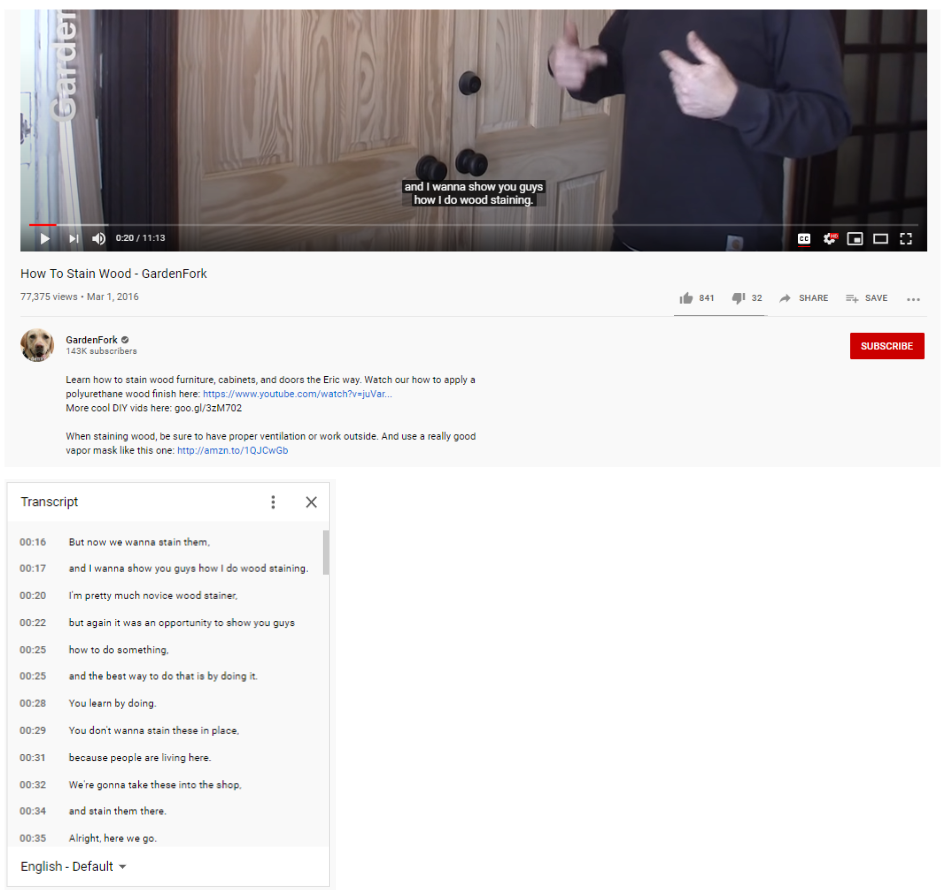
\includegraphics[width=\linewidth]{samplevideo.png}
  \caption{Sample Video}
  \label{fig:samplevideo}
\end{figure}


\subsection{Preprocessing}
\label{Preprocessing}

Due to diversity and complexity of our input data, a lot of our effort went into building a preprocessing pipeline out of blocks described in Figure \ref{fig:Preprocessing}. The format of CNN /Daily Mail stories, wikiHow articles, and howTo scripts is different. We invested substantial efforts into converting them to a format that can be used. For the convenience of other researchers who may want to use similar methodology, we shared the results of aligning them to the same fromat that can be training. 


\begin{figure}
  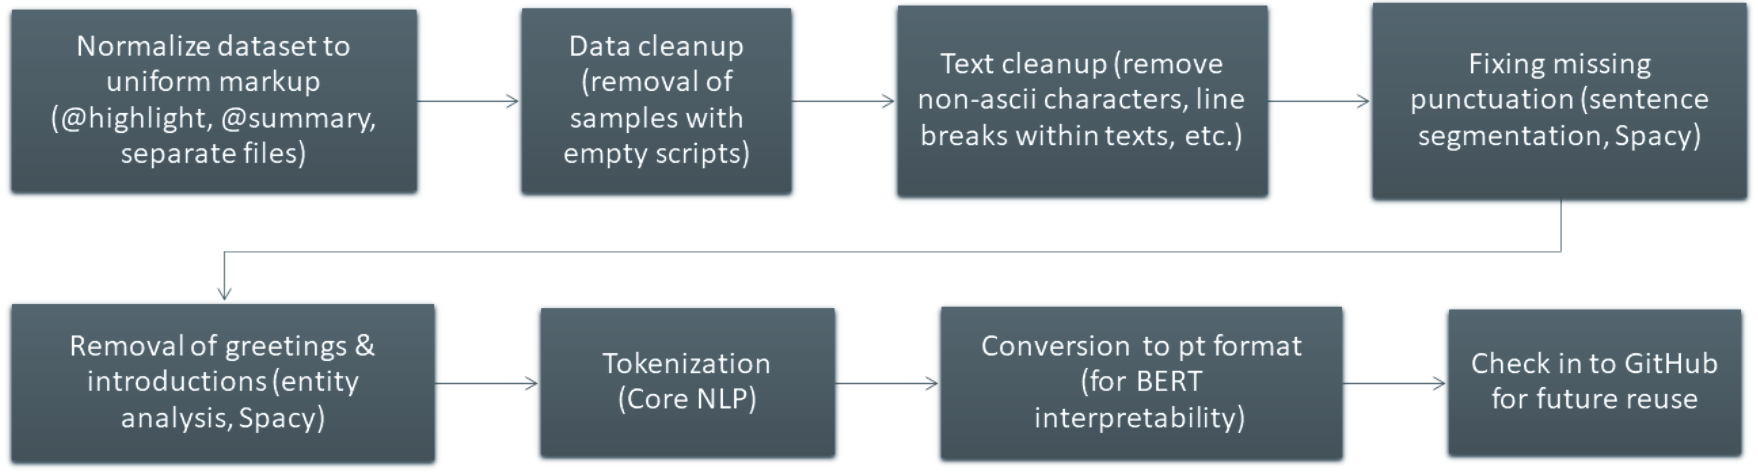
\includegraphics[width=\linewidth]{preprocessing.png}
  \caption{Preprocessing steps}
  \label{fig:Preprocessing}
\end{figure}

Another stream of work we have done at this stage is based on the heuristics observed during evaluation of results. Many scripts from YouTube (for the videos that we dupmed and HowTo100M dataset) have no punctuation, or it is not comprehensive. As a result, the model is misinterpreting text segment boundaries and produces low quality summaries or no summaries at all. With the help of Spacy library, we were able to fix this and restore sentence structures. 

We expected the differences in conversational style of the video scripts and writtent text of CNN stories (on which the models were pretrained) will impact quality of the output. In our first experiments, it manifested in a very distinct way. The model considered the first one-two sentences to be very important for summaries, and we ended up with getting many summaries looking like "hi!" and "hello, this is <first and last name>". It inspired us for implementing an improvement by using entity detection   \verb+spacy+ and \verb+nltk+ to remove introduction from the text that we feed to summarization model.  

The CNN/Daily Mail dataset has been preprocessed to remove news anchor introductions. For our Wikihow and How2 transcripts, we  did tokenization using the Stanford Core NLP toolkit and preprocessed the data in the same method used by (See et. al.).  


\subsection{Summarization models}

We used an  BertSum model created by Yang trained on CNN and Daily Mail [Yang]  for our paper. This paper has 2 separate models for Extractive and abstractive summarization. Extractive summarization is generally a binary classification task with labels indicating whether sentences should be included in the summary. Abstractive summarization, on the other hand, requires language generation capabilities to create summaries containing novel words and phrases not found in the source text. 

The architecture in the Figure \ref{fig:architecure} shows the BERTSUM model. It uses a novel documentation level encoder based on BERT which can encode a document and obtain representation for the sentences. CLS token is added to every sentence instead of just 1 CLS token in the original BERT model. Abstractive model uses an encoder-decoder architecture, combining the same pretrained BERT encoder with a randomly initialized Transformer decoder.The model uses a special technique where the encoder portion is almost kept same with a very low learning rate and create a separate learning rate for the decoder to make it learn better. 

\begin{figure}
  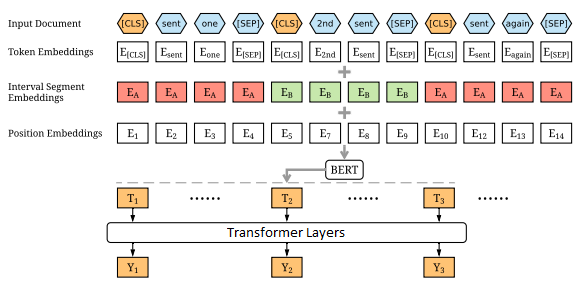
\includegraphics[width=\linewidth]{bertsumarchitecture.png}
  \caption{BERTSUM Architecture}
  \label{fig:architecure}
\end{figure}

In the beginning, we used a 4-GPU Linux machine and first trained on a small model with 10,000 steps using Extractive summarization. Extractive summarization uses BERT base uncased and took around 12 hours to train. We fine tuned the whole model including the BERT layer. We established the baseline by training on 5,000 samples from the How2 dataset. We tuned few hyper parameters with different steps, batch sizes and epochs sizes. Then, we added CNN/DM and full how2 dataset 3,097 samples from Wikihow with a 50,000 step size to the training set and got better summaries. 

Finally, we used the Abstractive summarization model and all the datasets(CNN/DM, Wikihow and how2 datasets) and trained for 210,000 steps in a specific order to get novel words and to get fluent summaries.This was done at the end as the abstractive model was very big and it took 4 days to train this model.These models are very demanding in terms of both memory and computational resources. The model has around 180 million parameters and has 2 Adam optimizers with $\beta_1$=0.9 and $\beta_2$ =0.999 for encoder and the decoder respectively. Encoder uses a learning rate of 0.002 and the decoder has a learning rate of 0.2. This is to make sure that the encoder is trained with more accurate gradients when the decoder is becoming stable.


\section{Experiments and Results}

\subsection{Training}
In order to create a generalizable model, we trained on large corpus of news. This allows our model to understand structured texts. We then introduced a comprehensive instructional text called Wikihow, which introduces the model to the how-to domain. Finally, we train and validate on the how-to dataset, narrowing the focus of the model to a selectively structured format. 

\begin{figure}
\centering
\begin{subfigure}{.5\textwidth}
  \centering
  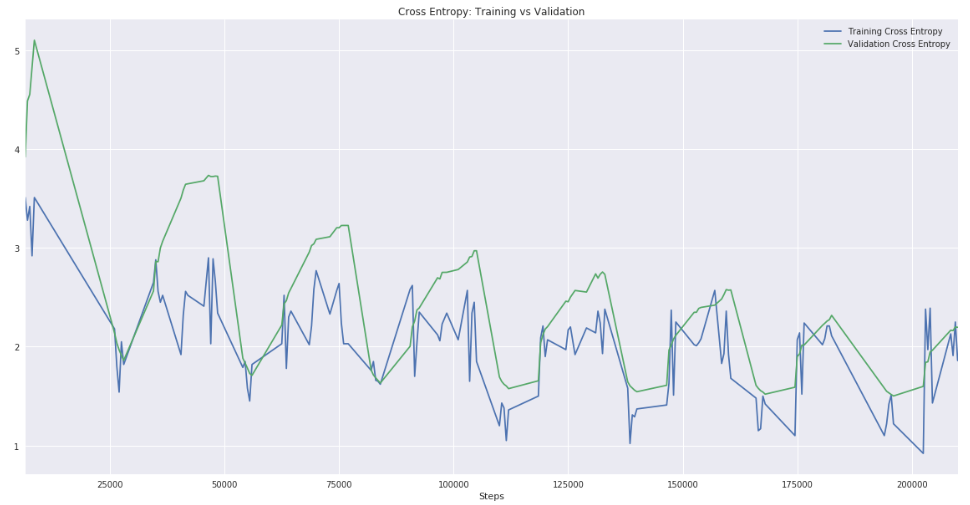
\includegraphics[width=\linewidth]{xent.png}
  \caption{Cross Entropy: Training vs Validation}
  \label{fig:xent}
\end{subfigure}%
\begin{subfigure}{.5\textwidth}
  \centering
  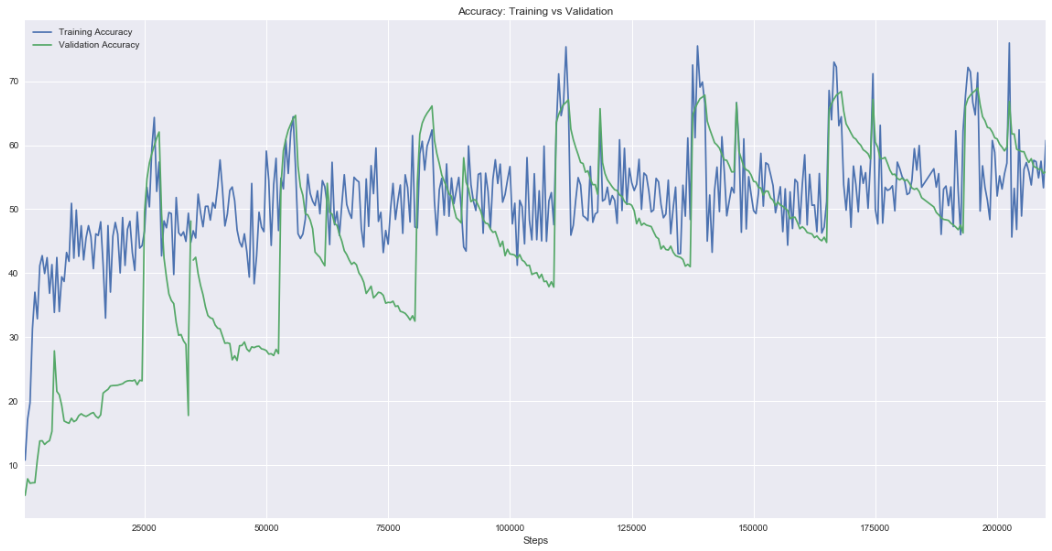
\includegraphics[width=\linewidth]{accuracy.png}
  \caption{Accuracy: Training vs Validation}
  \label{fig:accuracy}
\end{subfigure}
\caption{BertSum Abstractive Summarization: Model Performance}
\label{fig:modelperf}
\end{figure}

The cross entropy chart shows that the model is neither overfitting nor underfitting the training data. We want to see the lines meet and as seen here the model seems to be a good fit.Chart on the right shows the model’s accuracy metric on the Training and Validation sets. The model is validated using the how2 dataset against the training dataset that includes all 4 sources. The model improves as expected with more steps(or epochs). 


\subsection{Evaluation}
The BertSum model created by Yang trained on CNN and Daily Mail [Yang] resulted in SOTA rouge scores when applied to samples from those datasets. However, when tested on our How2 Test dataset, it gave very poor performance and a lack of generalization in the model (see Table~\ref{table1}). Looking at the data, we found that the model tends to pick the first one or two sentences for the summary. This can be explained by the fact that the first paragraph of a news article often captures the gits of it, which the model learned. However, in the case of our instructional videos, the first sentences would be a non-informative introduction, such as "Hi there! My name is ...". Based on that, we hypothesized that removing introuductions from the text will help improve ROUGE scores. Indeed, we got a few points better after applying  preprocessing described in the Section \ref{Preprocessing} above. Yet another improvement in the score was accomplished by taking advantage of one more observation: most curated summaries follow a template that starts with "Learn how ...". So, we added these two words in the beginning of the summary at post-processing stage. With all that, we still couldn't get higher than 22.5 ROUGE-1 F1 and 20 ROUGE-L F1. Reviewing scores and texts of individual summaries showed that the model is doing better on some topics, such as medicine, and worse on others, such as sports. Again, this makes sense for a model that is trained on news: it isn't reasonable for it to be good with yoga-specific terminology, while news about health care are very common.

So, in our next series of experiments, we used our own dataset for training. We were able to push the scores higher: by 4 for ROUGE-1 and 2.5 ROUGE-L F1 on the results with and without preprocessing, compared to the CNN-trained model. Current best results was accomplished with setting shuffling parameter to false when we train on CNN, HowTo Wiki, and HowTo Video scripts. Our results for videos have reached the level of the best scores for news [1]. However, there is still some  room for improvement, as more specialized model by [Shruti et.al.] claims to go above 50 ROUGE score.

\begin{table}
  \caption{Comparison of results}
  \label{table1}
  \centering
  \begin{tabular}{llll}
    \toprule
    \multicolumn{2}{c}{Experiment}                   \\
    \cmidrule(r){1-2}
    Model     & Pretraining Data     & Rouge-1 &Rouge-L\\
    \midrule
   1. PreSum  & CNN  and Daily Mail &18.08 &18.01    \\
 \midrule   
    2. PreSum with     & CNN  and Daily Mail & 20.51 &18.86     \\
      preprocessing    & & \\
\midrule
    3. PreSum with pre-     & CNN  and Daily Mail  & 22.47&20.07  \\
      and postprocessing    & & \\
\midrule
  4. PreSum  & How-To, WikiHow,   & 24.4 &21.45     \\
& CNN  and Daily Mail&\\
\midrule
  5. PreSum with  & How-To, WikiHow, & 26.32 &22.47    \\
postprocessing &CNN  and Daily Mail &\\
\midrule
 6. PreSum with  no shuffling& How-To, WikiHow, & 48.26 &44.02    \\
and more training data &CNN  and Daily Mail &\\
     \bottomrule
  \end{tabular}
\end{table}

In order to calculate ROUGE metrics, we used \verb+py-rouge+ package and initialized evaluator with a 100-word limit penalty as follows:
\begin{verbatim}
#nltk.download("punkt")
rouge_evaluator = rouge.Rouge(
    metrics=["rouge-n", "rouge-l"],
    max_n=4,
    limit_length=True,
    length_limit=100,
    length_limit_type="words",
    apply_avg=True,
    apply_best=False,
    alpha=0.5,  # Default F1_score
    weight_factor=1.2,
    stemming=True,
)
\end{verbatim}

We have observed examples of bad summaries with high ROUGE score, such as in Figure \ref{fig:funnysummary}, and good summaries with low ROUGE score. We believe that ROUGE is fine as a starting point for comparison, but the real evaluation of the output quality still requires human experts.

\begin{figure}
  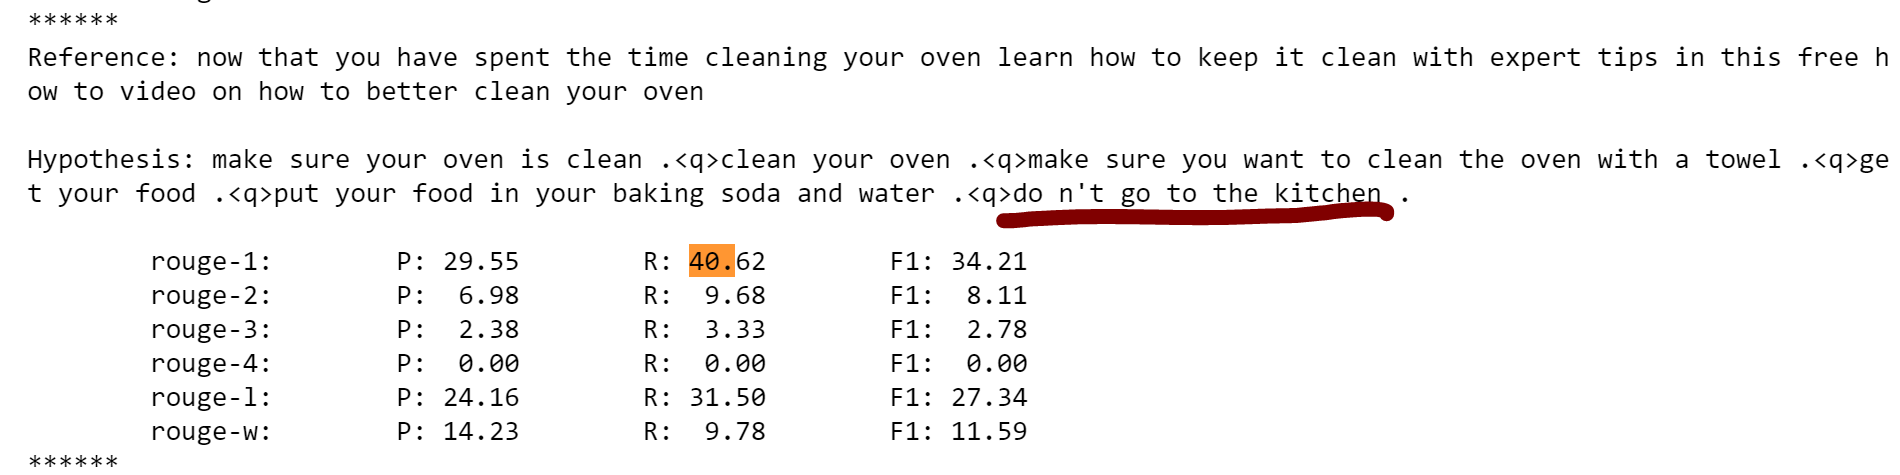
\includegraphics[width=\linewidth]{pic1.png}
  \caption{An example where ROUGE metric is confusing.}
  \label{fig:funnysummary}
\end{figure}

Even though the difference in ROUGE scores for the results on [1-3] are not drastically different from [4-5], the quality of summaries from the perspective of human judges is qualitatively different. From anecdotal paragraphs that made no sense, we went to very fluent and understandable video descriptions which give a clear idea about the content. We are still working on formalizing the expert evaluation framework and will provide more details on it in the next version of the paper. 

\section{Conclusion}
We are continuing to work on improving summarization for instructional videos, as measured by both ROUGE and human experts. By the end of the project, we hope to accomplish scores that are comparable to current SOTA, but more generalizable. We also plan to provide a more detailed analysis on correlations between features of a video (e.g. topic, length, number of likes) and the quality of summaries produced on our experiments, as well as a more detailed description of our expert evaluation process.


\section*{Broader Impact}

The contribution of our research is three-fold:
\begin{itemize}

\item We created and published a data set of how-to videos with time-tagged scripts, machine-generated summaries \footnote{https://github.com/alebryvas/berk266/ - it's not public repository yet, but we can provide access upon request}
\item We explored different combinations of data during training of summarization models and evaluated how they perform on instructional video scripts in different domains
\item We generalized  existing text summarization models to the scripts extracted from instructional videos  
\item We augmented ROUGE metrics [Chin-Yew Lin] for evaluation of the results with a framework for formalized expert assessment based on our research and criteria proposed by previous works \textit{[that's in work]}
\end{itemize}

At a high level, we hope that our analysis of transferability of summarization techniques from text to videos will have both practical and theoretical impacts by helping identify promising directions for future research.


\section*{References} 

{\bf We will allign the formatting of references for the final submission. Current list is accurate, but not standardized.}
\medskip



[1] Yang Liu, Mirella Lapata. Text Summarization with Pretrained Encoders.  \ (2019) URL. \url{https://arxiv.org/abs/1908.08345v2}

[2] Abigail See, Peter J. Liu, and Christopher D. Manning.\ (2017) Get to the point: Summarization with pointer-generator networks. In {\it Proceedings of the 55th Annual Meeting of the Association for Computational Linguistics \ (Volume 1: Long Papers)}, pages 1073-1083.

[3] Ilya Sutskever, Oriol Vinyals, and Quoc V Le. Sequence to sequence learning with neural networks.
 {\it Neural Information Processing Systems}, 2014. 

[4] Haoran Li, Junnan Zhu, Cong Ma, Jiajun Zhang, and Chengqing Zong. \ (2017). Multi-modal summarization for
asynchronous collection of text, image, audio and video. In {\it Proceedings of the 2017 Conference on Empirical
Methods in Natural Language Processing}, pages 1092–1102. Association for Computational Linguistics.

[5] Sanabria, R., Caglayan, O., Palaskar, S., Elliott, D., Barrault, L., Specia, L., and Metze, F. How2: A large-scale dataset for multimodal language understanding. {\it CoRR}, abs/1811.00347, 2018. URL. https://arxiv.org/abs/1811.00347

[6] Nenkova, A. (2005). Automatic text summarization of newswire: Lessons learned from the document understanding conference. In Proceedings of AAAI 2005, Pittsburgh, USA.

[7] Svore, K., Vanderwende, L., and Burges, C. (2007). Enhancing single-document summarization by combining RankNet and third-party sources. In Proceedings of the EMNLP-CoNLL, pages 448–457. [7, 8] 

[8] Yu-Hsiang Huang. Attention is all you need - pytorch. https://github.com/ jadore801120/attention-is-all-you-need-pytorch, 2018.

[9] Nima Sanjabi. Abstractive text summarization with attention-based mechanism. Master’s thesis, Universitat Politècnica de Catalunya, July 2018.

[10] Berna Erol, D-S Lee, and Jonathan Hull. 2003. Multimodal summarization of meeting recordings. In Multimedia and Expo, 2003. ICME’03. Proceedings. 2003 International Conference on, volume 3, pages III–25. IEEE.

[11] Dian Tjondronegoro, Xiaohui Tao, Johannes Sasongko, and Cher Han Lau. 2011. Multi-modal summarization of key events and top players in sports tournament videos. In Applications of Computer Vision (WACV), 2011 IEEE Workshop on, pages 471–478. IEEE

[12] Alexander M. Rush, Sumit Chopra, and Jason Weston. 2015. A neural attention model for abstractive sentence summarization. In Proceedings of the 2015 Conference on Empirical Methods in Natural Language Processing, pages 379–389. Association for Computational Linguistics.

[13] Shruti Palaskar, Jindrich Libovicky, Spandana Gella, Florian Metze. 2019. Multimodal Abstractive Summarization for How2 Videos. In Proceedings of the 57th Annual Meting of the Association for Computational Linguistics, pages 6587-6596. Association for Computational Linguistics.

[14] Antoine Miech, Dimitri Zhukov, Jean-Baptiste Alayrac, Makarand Tapaswi, Ivan Laptev, Josef Sivic. 2019. HowTo100M: Learning a Text-Video Embedding by Watching Hundred Million Narrated Video Clips. In ICCV 2019. https://arxiv.org/abs/1906.03327.



\end{document}
